\documentclass[10pt,twocolumn,letterpaper]{article}

% Pacotes basicos - maxima compatibilidade Windows
\usepackage{geometry}
\usepackage{times}
\usepackage{titlesec}
\usepackage{url}
\usepackage{graphicx,xcolor,comment,enumerate,multirow,multicol} 
\usepackage{amsmath,amsthm,amsfonts,amssymb,dsfont,mathtools}

% Configuracao da pagina
\geometry{
    letterpaper,
    left=0.75in,
    right=0.75in,
    top=0.75in,
    bottom=1in
}

% Configuracao das secoes
\titleformat{\section}[block]
{\normalfont\fontsize{10}{12}\bfseries}
{\thesection.}{0.5em}{}

% Remove numeracao das paginas
\pagestyle{empty}

% Configuracoes de espacamento
\setlength{\columnsep}{0.25in}
\setlength{\parindent}{0pt}
\setlength{\parskip}{6pt}

\begin{document}

% Titulo centralizado em coluna unica
\twocolumn[
\begin{center}
    {\fontsize{16}{19}\selectfont\bfseries 
    Experimento 1\\ Estudo dirigido sobre estruturas cristalinas}

    \vspace{12pt}
    
    {\fontsize{11}{13}\selectfont 
     Carlos Eduardo da S. Papa – 232013390, Robson Lima De Oliveira – 211067362, Ronan Cunha Freitas – 232013425 }

    \vspace{6pt}   

    {\fontsize{11}{13}\selectfont 
    Turma 01}
    
    \vspace{18pt}
\end{center}
]

\section{OBJETIVOS}

\begin{figure}
    \centering
    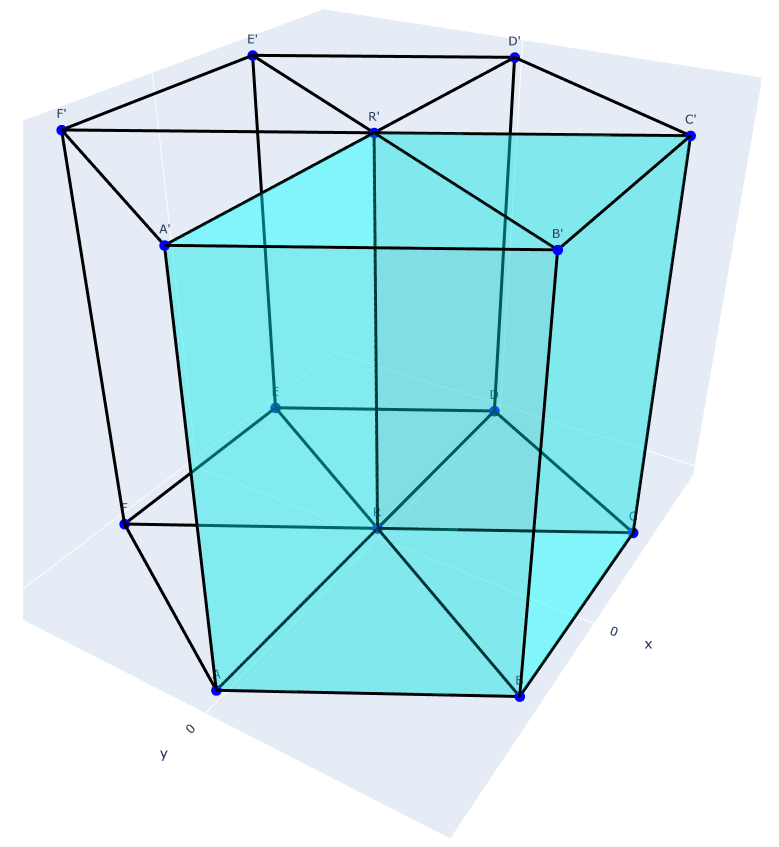
\includegraphics[width=5cm]{PrimitiveCell.png}
    \caption{Célula primitiva da célula hexagonal simples (HS)}
    \label{fig:label}
\end{figure}

\hspace{1cm} Colocar TEXTO.

\vspace{.75cm}

\section{INTRODUCAO}
\hspace{1cm}  Colocar TEXTO.

\vspace{.75cm}

\section{MATERIAIS UTILIZADOS}

\hspace{1cm} Colocar TEXTO.

\vspace{.75cm}

\vspace{.75cm}

\section{PROCEDIMENTOS EXPERIMENTAIS}

\hspace{1cm} Colocar TEXTO.

\vspace{.75cm}

\section{RESULTADOS EXPERIMENTAIS}

\hspace{1cm} Colocar TEXTO.

\vspace{.75cm}

\section{ANALISE DOS RESULTADOS EXPERIMENTAIS}

\hspace{1cm} Colocar TEXTO.

\vspace{.75cm}

\section{REFERENCIAS BIBLIOGRAFICAS}

\small
\begin{enumerate}
    \item CESCHIN, Artemis M. Apostila de materiais eletricos e magneticos.
    
    \item \url{https://mateck.com/en/content/119-selen-34se78} "Selenium (Se) - Mateck"
    
    \item \url{https://www.periodic-table.org/Selenium-crystal-structure/} "Selenium - Crystal Structure"
    
    \item \url{https://www.isoflex.com/selenium-se} "ISOFLEX USA - Selenium"
    
    \item \url{https://www.espimetals.com/index.php/technical-data/253-Tellurium.com} "Tellurium - ESPI Metals"
    
    \item \url{https://www.chemicalbook.com/article/tellurium-crystal.htm} "Tellurium Crystal Chemicalbook"
    
    \item \url{https://www.osti.gov/etdeweb/biblio/275148} "The crystal structure and optical activity of tellurium"
    
    \item \url{https://en.institut-seltene-erden.de/seltene-erden-und-metalle/strategische-metalle-2/tellur/} "Tellurium Price, Occurrence, Extraction and Use"
    
    \item \url{https://www.periodic-table.org/tellurium-crystal-structure/} "Tellurium - Crystal Structure"
    
    \item \url{https://en.wikipedia.org/wiki/Tellurium} "Tellurium"
    
    \item \url{https://www.geeksforgeeks.org/chemistry/graphite/} "Graphite - GeeksforGeeks"
    
    \item \url{https://www.infogalactic.com/info/Graphite} "Graphite - Infogalactic"
    
    \item \url{https://unacademy.com/content/jee/study-material/chemistry/structure-of-carbon-allotrope/} "Structure of Carbon Allotrope"
\end{enumerate}

\end{document}